\documentclass{beamer}
\usetheme{Frankfurt}

\usepackage{listings}

\title{Multilevel Security}
\subtitle{Lecture 10 \\ Computer Security DD2395}
\author[R. Guanciale]{
  Roberto Guanciale\\
  robertog@kth.se
}
\date{2015-12-03}
\begin{document}

\begin{frame}[plain]
  \titlepage
\end{frame}

\begin{frame}{Computer Security Models}
  \begin{itemize}
  \item all complex systems have eventually revealed flaws (design)
  \item extraordinary difficult to implement (hw/sw) the design
    without introducing bugs
  \item methods to prove that a design satisfies a set of security requirements
  \item methods to prove that the implementation conforms the design
  \item today: models, their enforcement (verification), trusted systems
  \end{itemize}
\end{frame}

\begin{frame}{Computer Security Models}
``A design without specification cannot be right or wrong,
  it can only be surprising!''
  \\
  Young
  \\
  Use formal machinery to state properties, describe specifications
  and analyze designs
\end{frame}


\begin{frame}{Access controls}
  Formalize restrictions of accesses to resources\\[10pt]
\begin{center}
  \begin{tabular}{|c|c|c|c|}
    \hline
    M & file1 & file2 & directory \\
    \hline
    user1 & r,w & r & r,w,x \\
    \hline
    user2 & r,w & - & r \\
    \hline
    user3 & r & - & r,w \\
    \hline
  \end{tabular}
\end{center}
  \begin{itemize}
  \item $s$ can do $op$ on $o$ if $op \in M[s,o]$
  \item Discretionary AC: ``owner'' sets permissions
    \begin{itemize}
      \item users make mistakes
    \end{itemize}
  \item<2-> Mandatory AC: system-wide policy decides
    \begin{itemize}
      \item DAC can not give more access than MAC
    \end{itemize}
  \end{itemize}
\end{frame}

\begin{frame}{Multi-Level Security}
  \begin{itemize}
  \item MLS uses ordered security classes, e.g.
    \begin{itemize}
    \item hardware: supervisor/user CPU modes
    \item software: superuser/user Linux/Windows
    \item military: top secret, secret, confidential, restricted, unclassified 
    \item business: strategic, sensitive, confidential, public
    \end{itemize}
  \end{itemize}
\end{frame}

\begin{frame}{Bell-La Padula (BLP) Model}
  \begin{itemize}
  \item developed in 1970s
  \item formal access control model
  \item subjects and objects have a \alert{security class}
    \begin{itemize}
    \item subject has a \alert{security clearance} level
    \item object has a \alert{security classification} level
    \item class control how subject may access an object
    \end{itemize}
  \end{itemize}
\end{frame}

\begin{frame}{Bell-La Padula (BLP) Model}
  \begin{itemize}
  \item security levels (partially) ordered
    \begin{itemize}
    \item $L0 < L1 < L2 < L3$
    \item $L0 < L1$, $L0 < L2$, $L1 < L3$, $L2 < L3$
    \end{itemize}
  \item captures \alert{confidentiality}
    \begin{itemize}
      \item information can not flow from more secure to 
        less secure levels
    \end{itemize}
    \item access modes:
    \begin{itemize}
    \item $r$: read
    \item $a$: append
    \item $w$: write
    \item $x$: execute
    \end{itemize}
  \end{itemize}
\end{frame}

\begin{frame}{BLP State}
  \begin{itemize}
  \item state is a tuple $(b,M,f, H)$
  \item current access set $b = \{(s_1,o_1,a_1),\dots,(s_n,o_n,a_n)\}$
    \begin{itemize}
    \item $(s_i,o_i,a_i)$: the subject $s_i$ is exercising the access
      $a_i$ to the object $o_i$
    \end{itemize}
  \item current access matrix $M$
    \begin{itemize}
    \item $s$ can do $op$ on $o$ if $op \in M[s,o]$
    \end{itemize}
  \item level functions $f=(f_o, f_s, f_c)$
    \begin{itemize}
      \item $f_o(o_j)$: classification level of object $o_j$
      \item $f_s(s_j)$: security clearance (max sec.level) of subject $s_j$
      \item $f_c(s_j)$: current sec.level of subject $s_j$
        ($f_c(s_j) \leq f_s(s_j)$)
    \end{itemize}
    \item $H$ is an object hierarchy respecting the
      security level partial order
  \end{itemize}
\end{frame}

\begin{frame}{BLP: Simple Security}
  \begin{itemize}
  \item ss-property: no read up
  \item a subject may read only if it has at least as high security
    clearance as the object
  \item $(s_i, o_i, read) \in b$ then
    $f_c(s_i) \geq f_o(o_i)$
  \item<2-> \alert{confidentiality}: information can not flow from more secure to 
        less secure levels
  \item<3-> is ss-property sufficient to guarantee confidentiality?
  \end{itemize}
\end{frame}

\begin{frame}{BLP: Simple Security}
  \begin{center}
    \only<1>{
    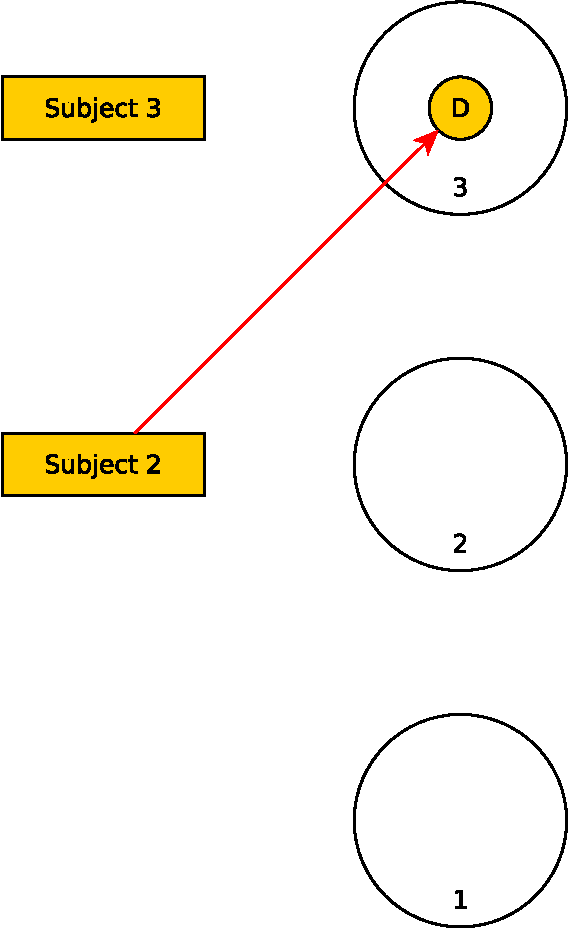
\includegraphics[width=0.4\linewidth]{blp-ss1}
  }
    \only<2>{
    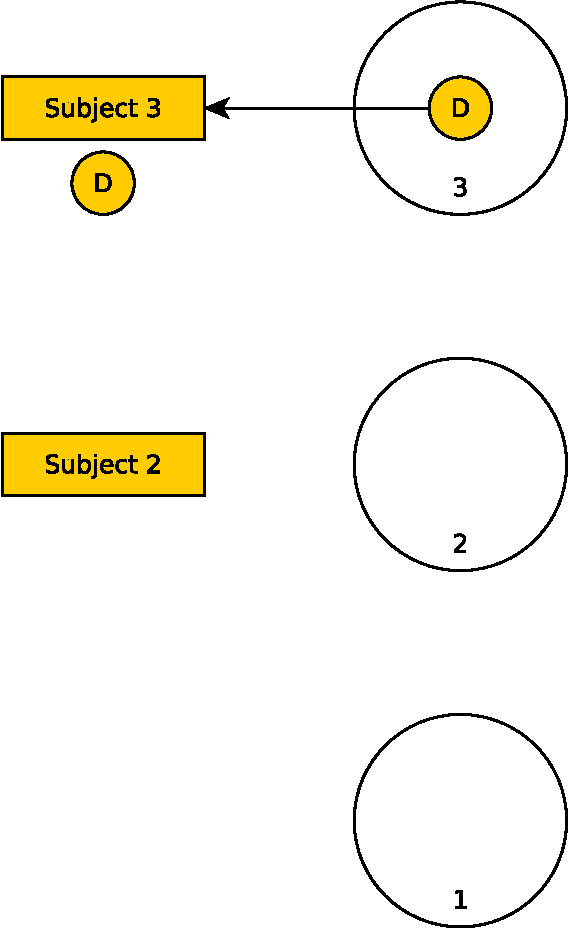
\includegraphics[width=0.4\linewidth]{blp-ss2}
  }
    \only<3>{
    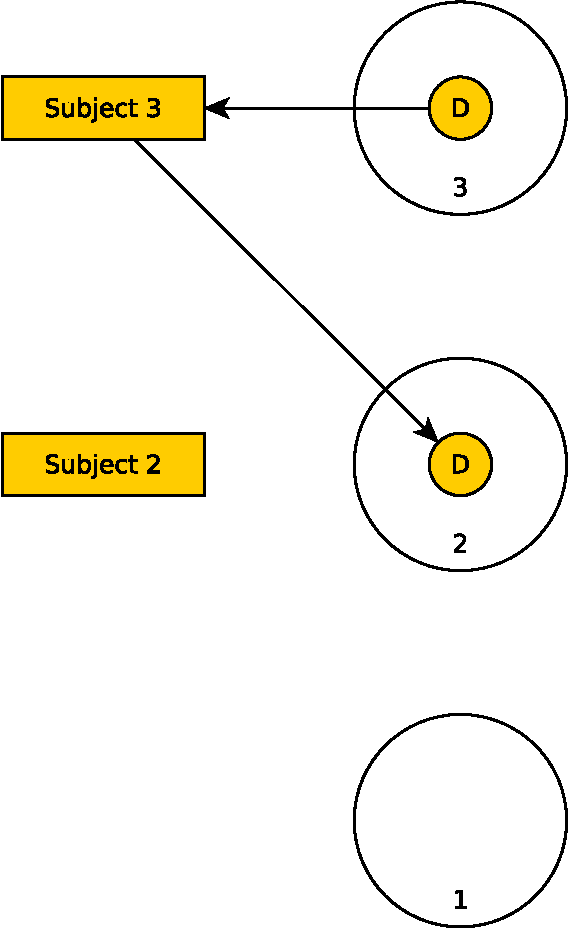
\includegraphics[width=0.4\linewidth]{blp-ss3}
  }
    \only<4>{
    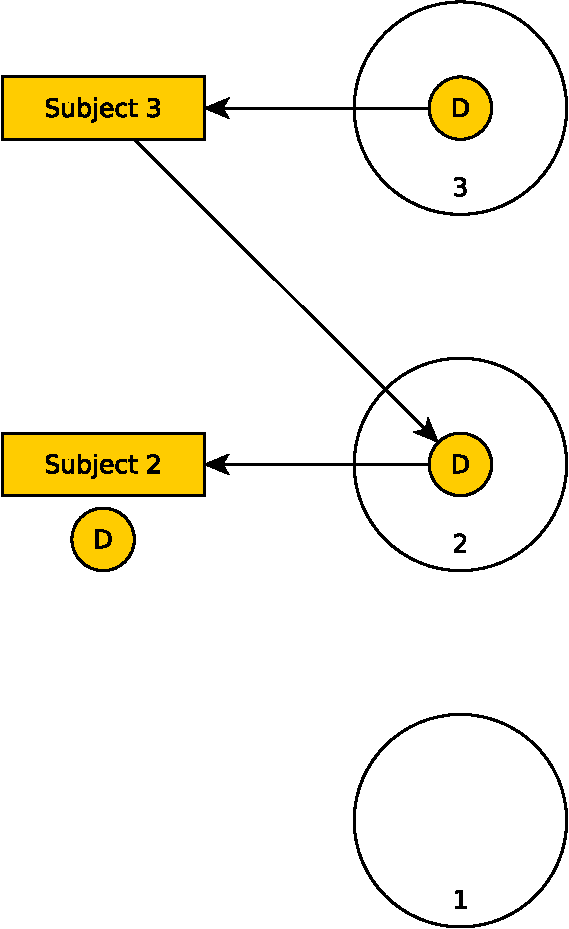
\includegraphics[width=0.4\linewidth]{blp-ss4}
  }
  \end{center}
\end{frame}

\begin{frame}{BLP: Star Security}
  \begin{itemize}
  \item $*$-property: no write down
  \item a subject may write (append) only if it has equal (at most as)  security
    clearance as the object
  \item $(s_i, o_i, write) \in b$ then
    $f_c(s_i) = f_o(o_i)$
  \item $(s_i, o_i, append) \in b$ then
    $f_c(s_i) \leq f_o(o_i)$
  \item with the ss-property implies that:
    \begin{itemize}
      \item can't read a high-level object while writing a lower-level
        object
      \item $(s_i, o'_i, read) \in b$ then
        $f_o(o') \leq f_o(o)$
    \end{itemize}
  \end{itemize}
\end{frame}

\begin{frame}{BLP: Discretionary Security}
  \begin{itemize}
  \item ds-property: discretionary access control
  \item only (owner) permitted accesses are allowed
  \item $(s_i, o_i, a_i) \in b$ then
    $a_i \in M[s_i, o_i]$
  \end{itemize}
\end{frame}


\begin{frame}{BLP Rules}
  \begin{itemize}
    \item get access: add a triple $(s,o,a)$ to $b$
    \item release access: remove triple from $b$
    \item change object level ($f_o$)
    \item change current level of subject ($f_c$)
    \item give access permission (M) 
    \item rescind access permission (M) 
    \item object hierarchy: create an object: add a leaf,
      delete a group of objects (H)
  \end{itemize}
\end{frame}

\begin{frame}{BLP: system security}
  \begin{itemize}
  \item a state $S=(b,M,f)$ is secure if and only if 
    \begin{itemize}
      \item $ss-property(S)$
      \item $*-property(S)$
      \item $ds-property(S)$
    \end{itemize}
  \item a transition $S \rightarrow S'$ is secure if
    both $S$ and $S'$ are secure
  \item a system is secure if the initial state(s) is secure
    and all transitions are secure
  \end{itemize}
\end{frame}

%initial
%7-Create an object
%5-Give access permission
%1-Get access

\begin{frame}[t]{BLP: Example}
  \begin{center}
    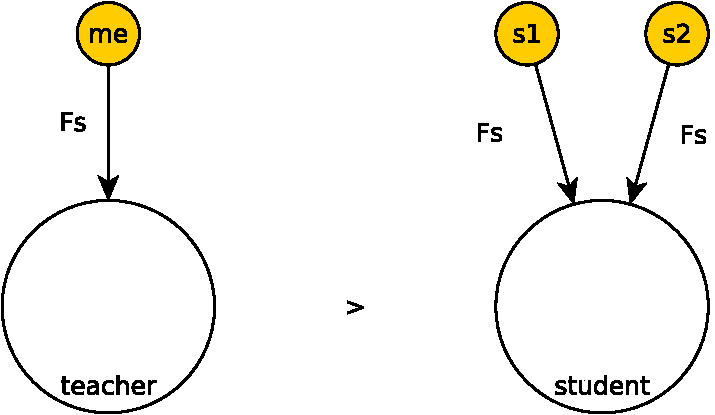
\includegraphics[width=0.5\linewidth]{ex1}
  \end{center}
\end{frame}
\begin{frame}[t]{BLP: Example, D1 is the exam template}
  \begin{center}
    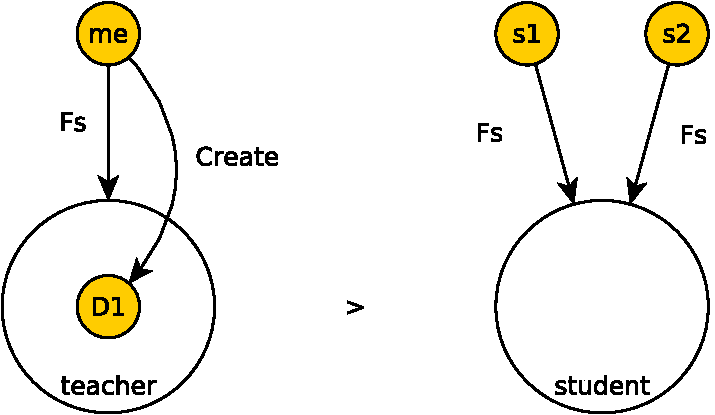
\includegraphics[width=0.5\linewidth]{ex2}
  \end{center}
\begin{enumerate}
  \item Create an object
\end{enumerate}
\end{frame}
\begin{frame}[t]{BLP: Example, D1 is the exam template}
  \begin{center}
    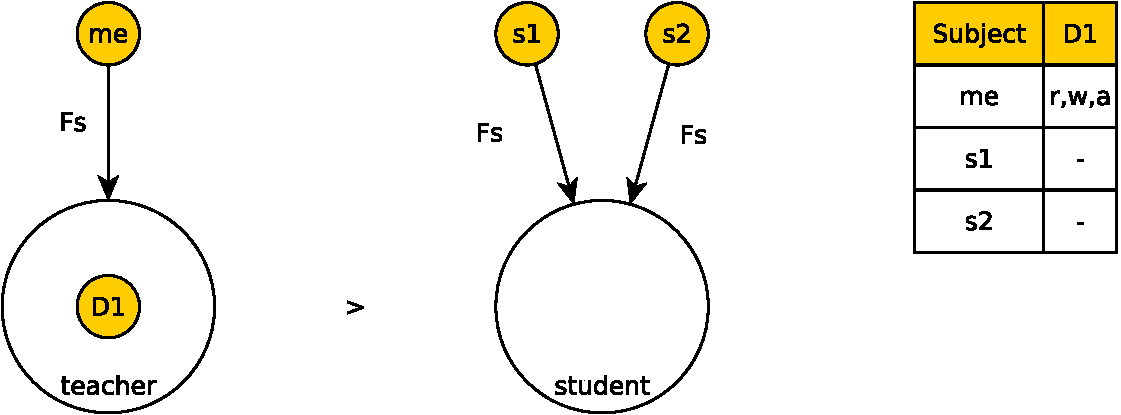
\includegraphics[width=0.8\linewidth]{ex3}
  \end{center}
\begin{enumerate}
  \item Give access permission
\end{enumerate}
\end{frame}
\begin{frame}[t]{BLP: Example, D1 is the exam template}
  \begin{center}
    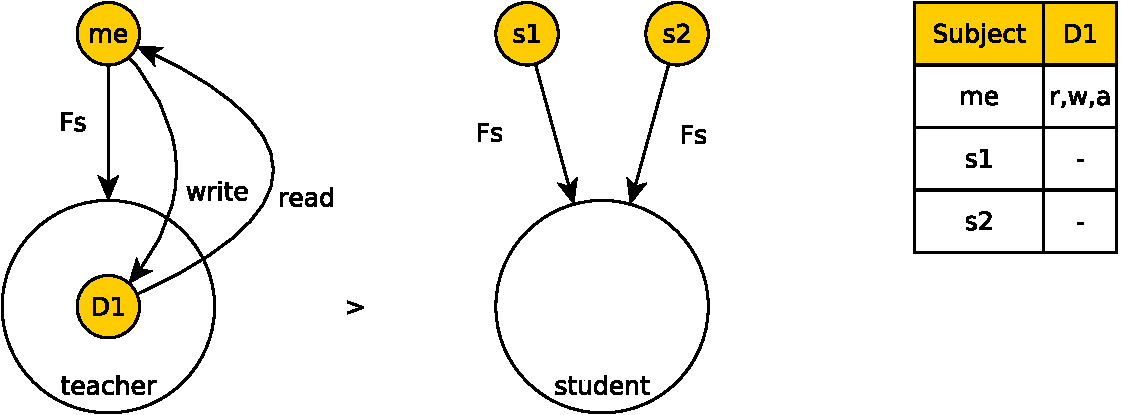
\includegraphics[width=0.8\linewidth]{ex4}
  \end{center}
\end{frame}
\begin{frame}[t]{BLP: Example, D1 is the exam template}
  \begin{center}
    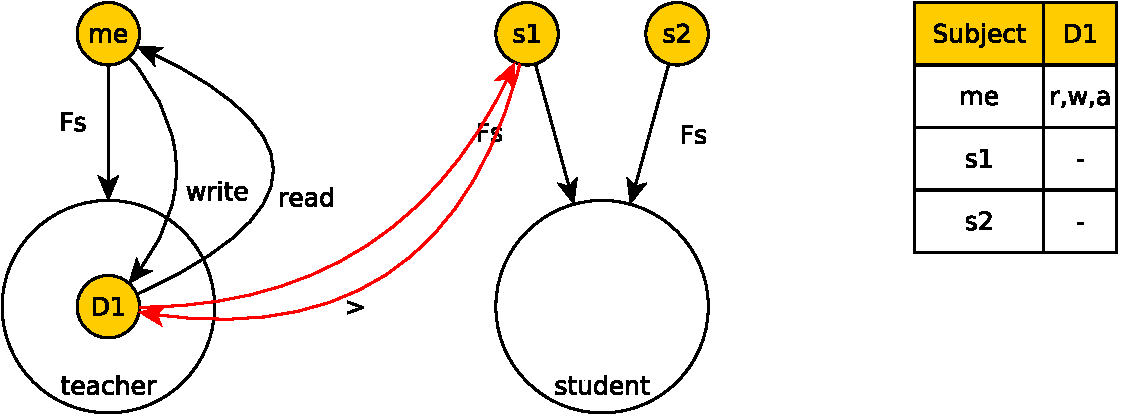
\includegraphics[width=0.8\linewidth]{ex5}
  \end{center}
\end{frame}
\begin{frame}[t]{BLP: Example, D2 is the lab S report}
  \begin{center}
    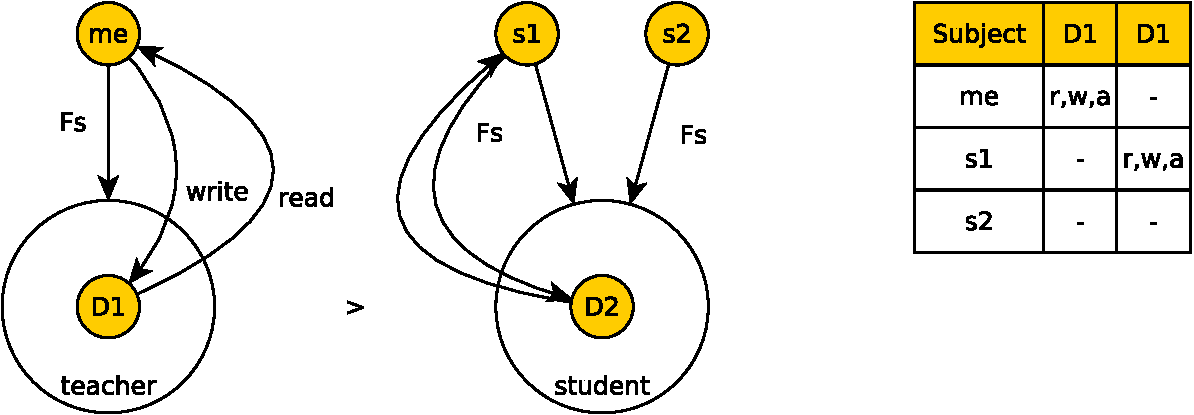
\includegraphics[width=0.9\linewidth]{ex6}
  \end{center}
\begin{enumerate}
  \item Create an object
  \item Give access permission
\end{enumerate}
\end{frame}
\begin{frame}[t]{BLP: Example, D2 is the lab S report}
  \begin{center}
    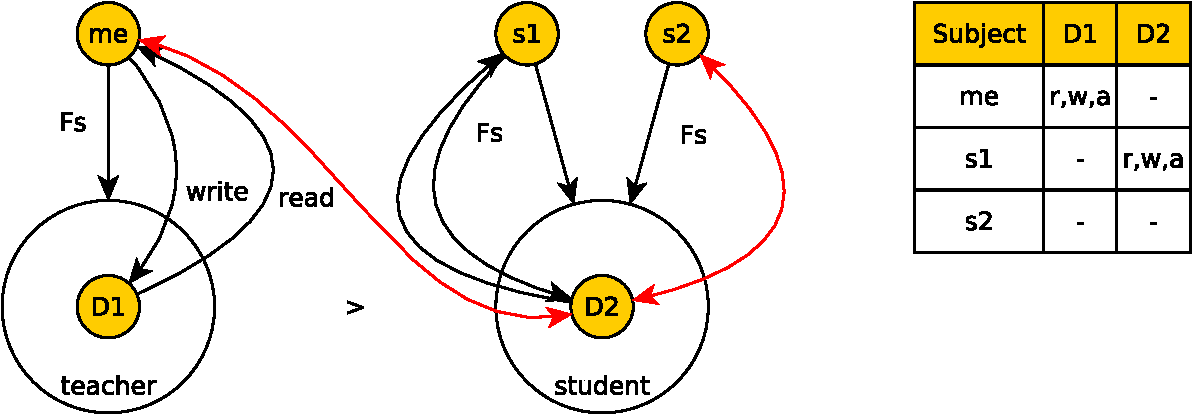
\includegraphics[width=0.9\linewidth]{ex7}
  \end{center}
\end{frame}

\begin{frame}[t]{BLP: Example, D2 is the lab S report}
  \begin{center}
    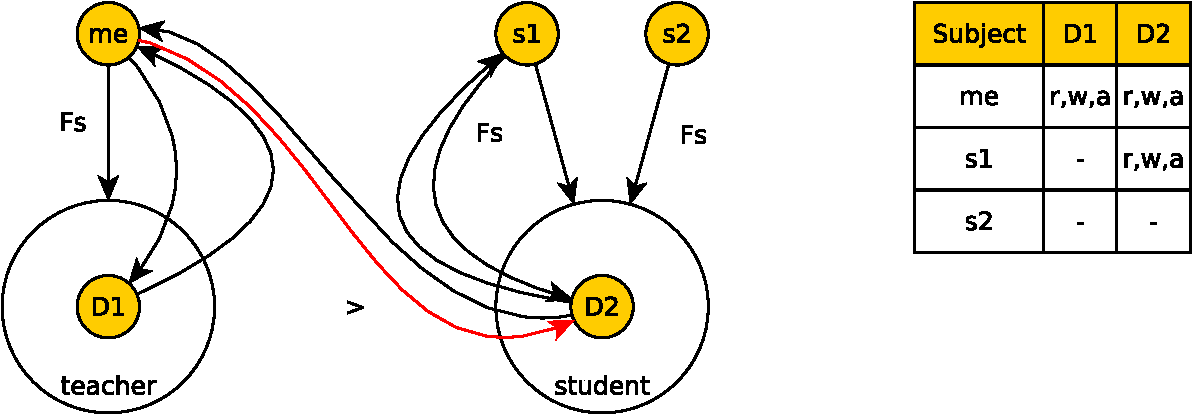
\includegraphics[width=0.8\linewidth]{ex8}
  \end{center}
\begin{enumerate}
  \item Give access permission
\end{enumerate}
\end{frame}

\begin{frame}[t]{BLP: Example, C2 contains the comments to the report}
  \begin{center}
    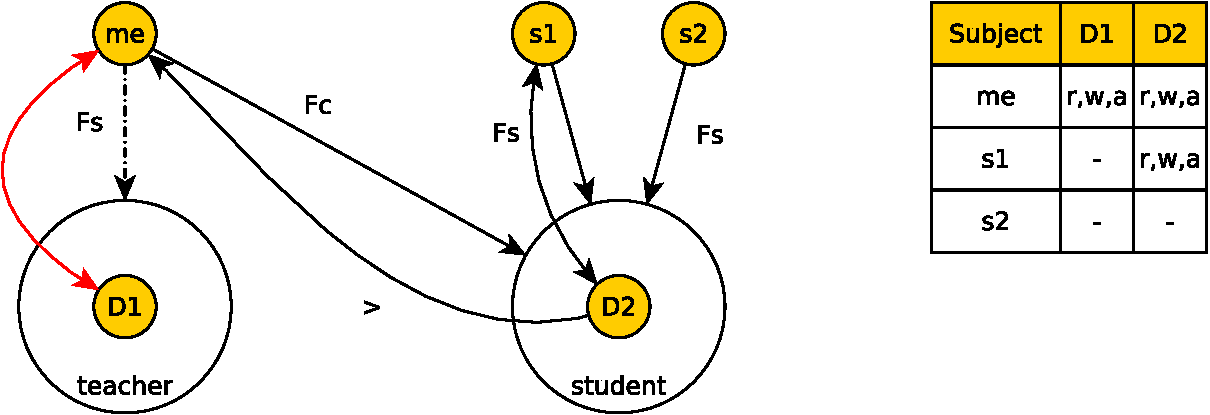
\includegraphics[width=0.8\linewidth]{ex9}
  \end{center}
\begin{enumerate}
  \item Change current level
\end{enumerate}
\end{frame}

\begin{frame}[t]{BLP: Example, C2 contains the comments to the report}
  \begin{center}
    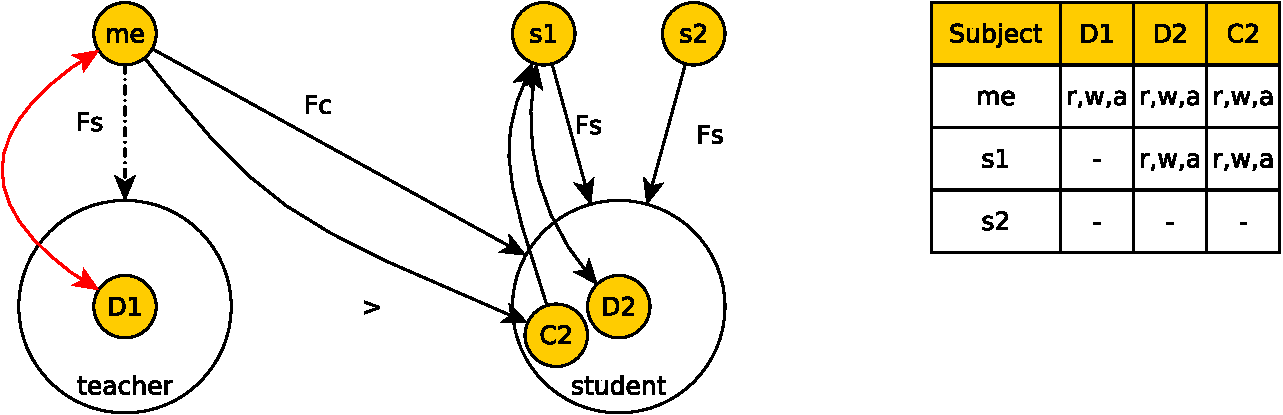
\includegraphics[width=0.8\linewidth]{ex10}
  \end{center}
\begin{enumerate}
  \item Create an object
  \item Give access permission
\end{enumerate}
\end{frame}

\begin{frame}[t]{BLP: Example, D2 contains the exam for the student}
  \begin{center}
    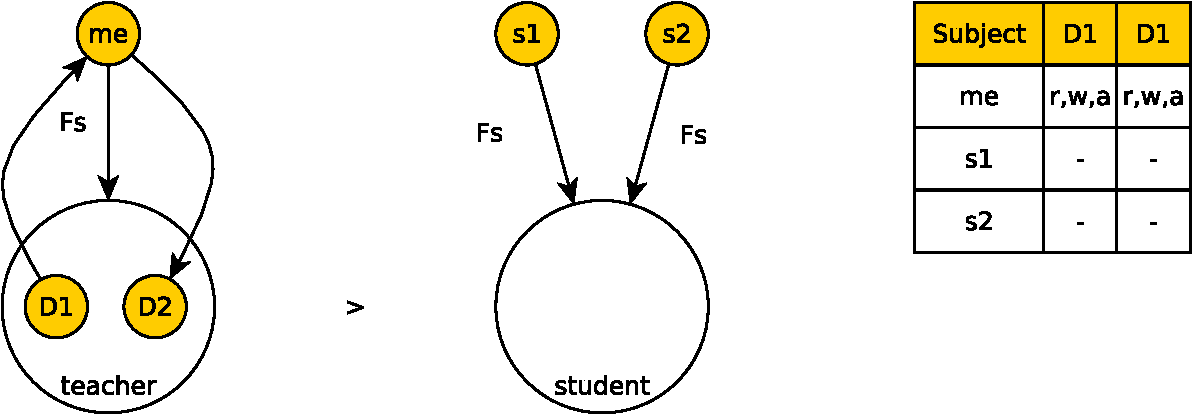
\includegraphics[width=0.8\linewidth]{ex11}
  \end{center}
\begin{enumerate}
  \item Create an object
  \item Give access permission
\end{enumerate}
\end{frame}

\begin{frame}[t]{BLP: Example, D2 contains the exam for the student}
  \begin{center}
    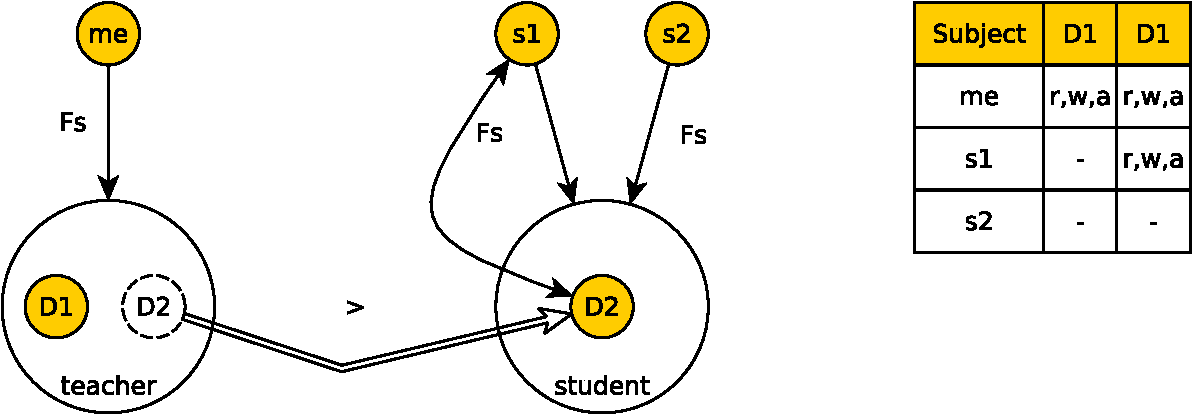
\includegraphics[width=0.8\linewidth]{ex12}
  \end{center}
\begin{enumerate}
  \item Give access permission
  \item Change object level (declassification)
\end{enumerate}
\end{frame}

\begin{frame}{BLP Limitation}
  \begin{itemize}
    \item No internal provision for downgrading
    \item Classification creep by consolidation of 
      documents from different sources and levels
    \item \alert{trusted subjects}: set of subjects which are 
      allowed to break *-property (assuming they always 
      ``clean'' the information)
    \item ``trusted''  means ``can hurt you''
    \item ``trustworthy'' means ``verified not to hurt you''
  \end{itemize}
\end{frame}


\begin{frame}{Biba Integrity Model}
  \begin{itemize}
    \item deals with integrity
    \item uses integrity levels
    \item reverses permitted flows: 
      no ``dirty'' low-integrity info may flow to ``clean'' 
      high-level info, but other way OK
  \end{itemize}
\end{frame}

\begin{frame}{Biba Policy}
  \begin{itemize}
    \item simple integrity
      \begin{itemize}
      \item no write up
      \item $(s_i, o_i, write) \in b$ then
        $i_c(s_i) \ge i_o(o_i)$
      \end{itemize}
    \item integrity confinement
      \begin{itemize}
      \item no read down
      \item $(s_i, o_i, read) \in b$ then
        $i_c(s_i) \le i_o(o_i)$
      \end{itemize}
    \item invocation property
      \begin{itemize}
      \item invocation property
      \item $(s_i, s_j, invoke) \in b$ then
        $i_c(s_i) \ge i_c(s_j)$
      \end{itemize}
  \end{itemize}
\end{frame}

\begin{frame}{Chinese Wall model}
  \begin{itemize}
    \item inspired by commercial applications
    \item conflict of interest
    \item hierarchical
      \begin{itemize}
      \item objects ($O \in DS$): individual item of information
      \item dataset ($DS \in CI$): all objects that concern the same corporation
      \item conflict of interest class ($CI$): corporations in competition
      \end{itemize}
    \item information can not flow between two corporations in competition
  \end{itemize}
\end{frame}

\begin{frame}{Chinese Wall policy}
  \begin{itemize}
    \item keep access list $H$
    \item simple security rule
      \begin{itemize}
        \item $(s_i, o_i, read) \in b$ then $ss(s_i,o_i)$ where
        \item $\exists o_j \in DS(O). (s_i, o_j, read) \in H$ or
        \item $\not \exists o_j \in CI(O). (s_i, o_j, read) \in H$
        \item read allowed if the subject already accesses the dataset
          or he has not accessed any information from the CI
      \end{itemize}
    \item $*$-property rule
      \begin{itemize}
        \item $(s_i, o_i, write) \in b$ then
        \item $ss(s_i,o_i)$
        \item $\forall o_j.ss(s_i,o_j) \Rightarrow DS(o_j) = DS(o_i)$
        \item write allowed if the subject can read the object and can
          not read outside the DS
      \end{itemize}
  \end{itemize}
\end{frame}

\begin{frame}{Chinese Wall: Example}
  \begin{center}
\only<1>{
    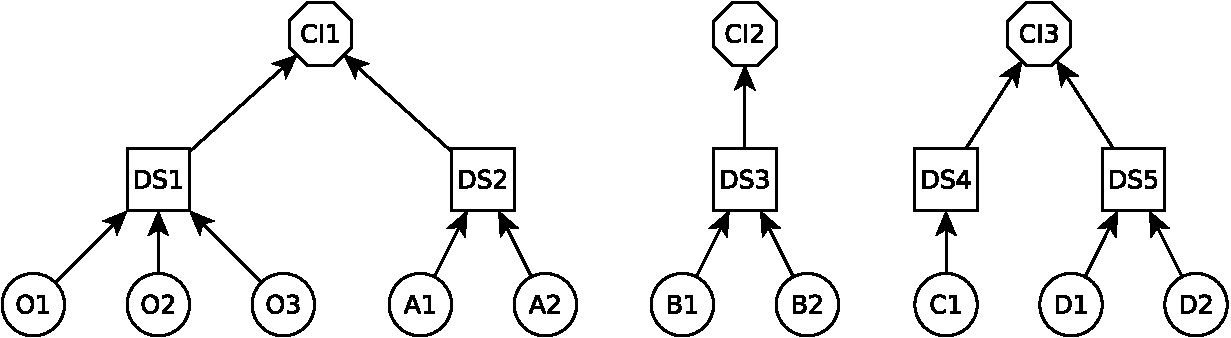
\includegraphics[width=0.8\linewidth]{cw1}
}
\only<2>{
    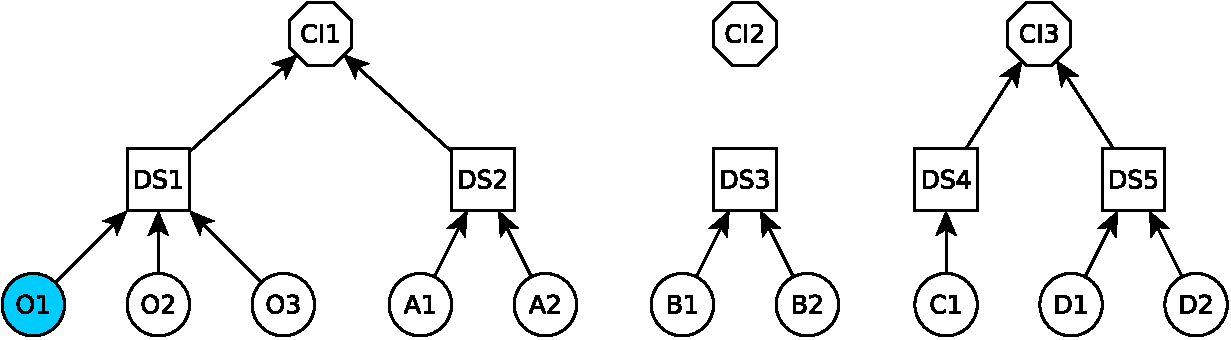
\includegraphics[width=0.8\linewidth]{cw2}
}
\only<3>{
    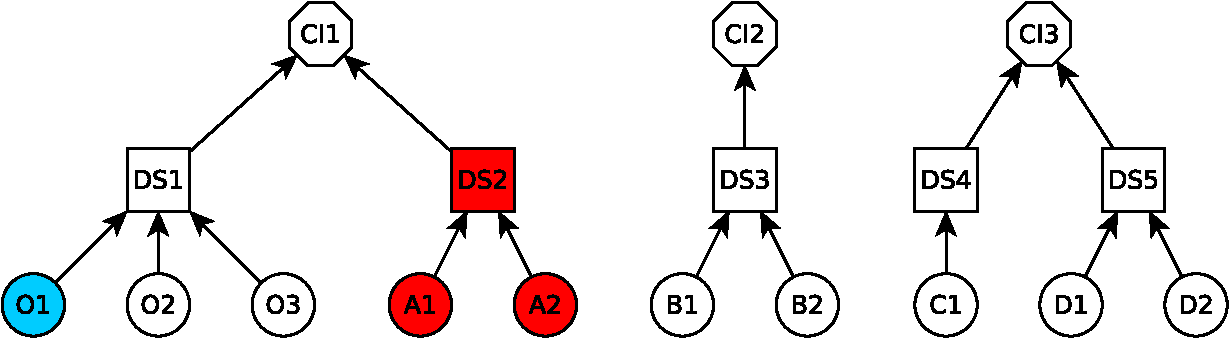
\includegraphics[width=0.8\linewidth]{cw3}
}
\only<4>{
    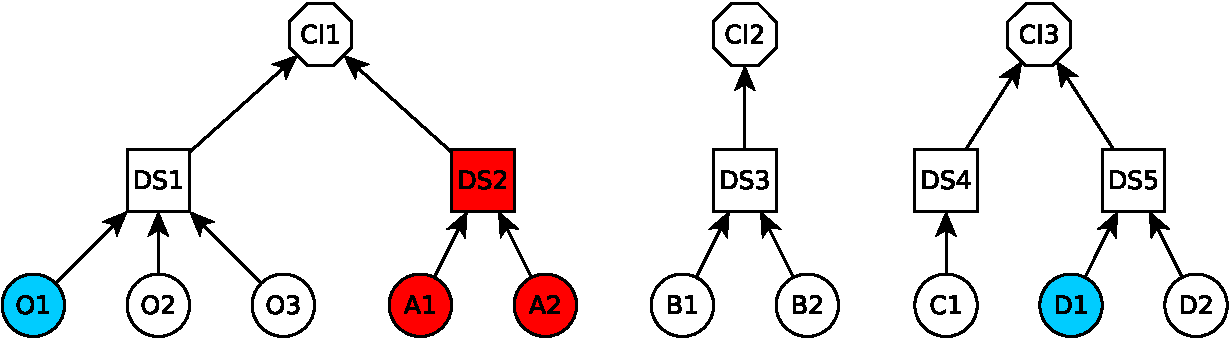
\includegraphics[width=0.8\linewidth]{cw4}
}
\only<5>{
    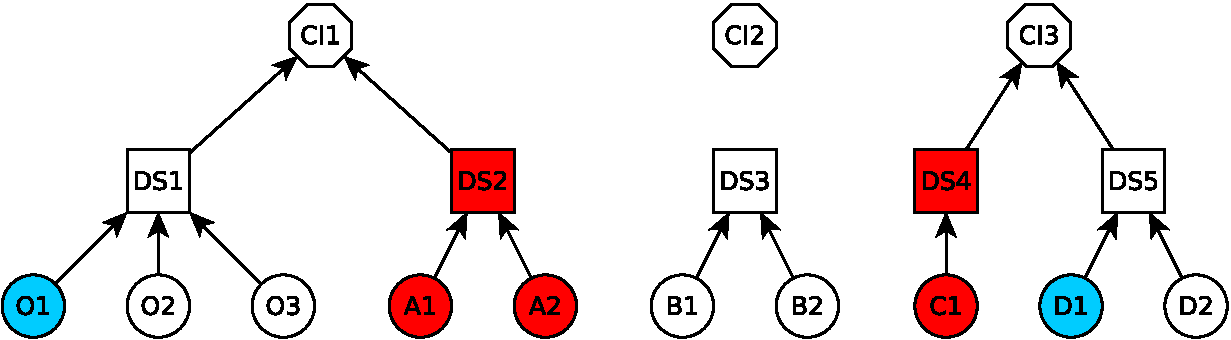
\includegraphics[width=0.8\linewidth]{cw5}
}
  \end{center}
\end{frame}

\begin{frame}{Reference Monitor}
  \begin{itemize}
  \item complete mediation
  \item isolation
  \item verifiability
  \end{itemize}
  \begin{center}
\only<1>{
    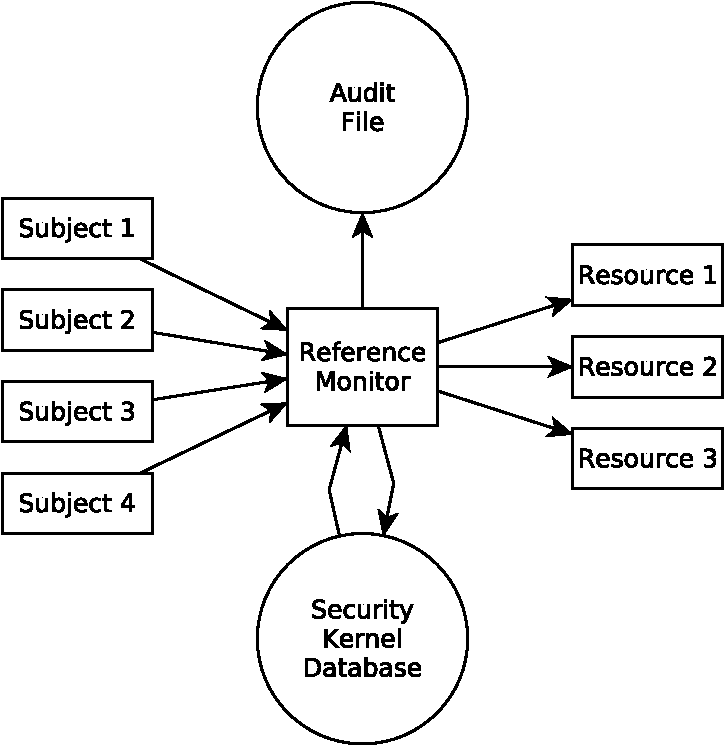
\includegraphics[width=0.4\linewidth]{referenceMonitor}
}
\only<2>{
    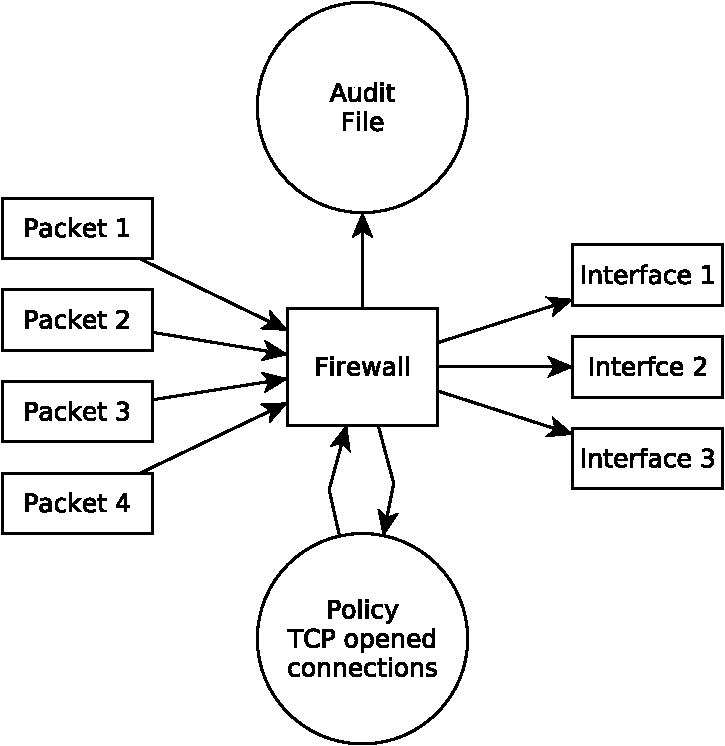
\includegraphics[width=0.4\linewidth]{fw}
}
\only<3>{
    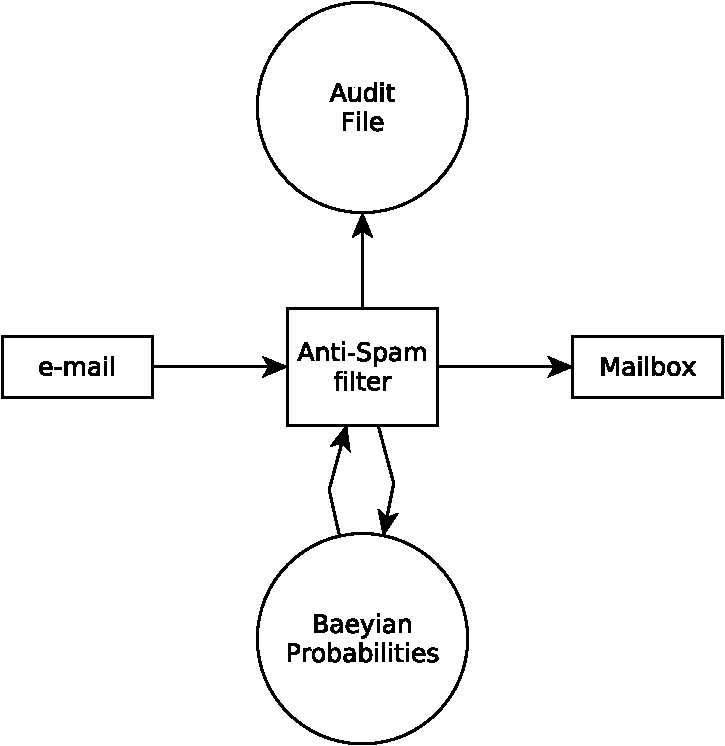
\includegraphics[width=0.4\linewidth]{antispam}
}
\only<4>{
    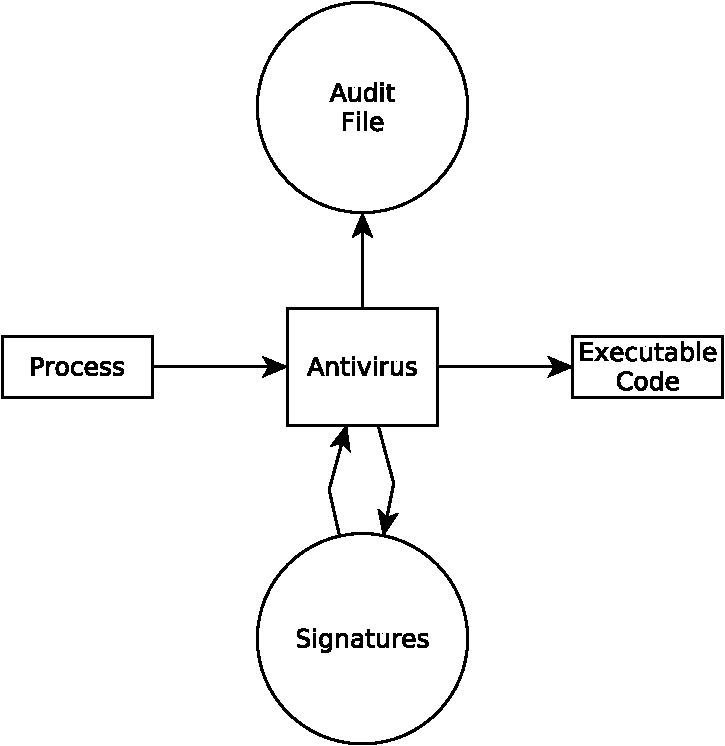
\includegraphics[width=0.4\linewidth]{antivirus}
}
  \end{center}
\end{frame}

\begin{frame}{MLS and (relational)-databases}
  \only<1>{
  \begin{center}
    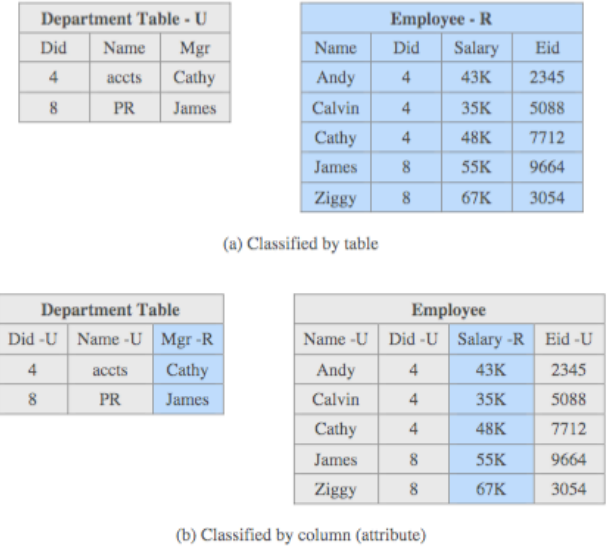
\includegraphics[width=0.8\linewidth]{database1}
  \end{center}
}
  \only<2>{
  \begin{center}
    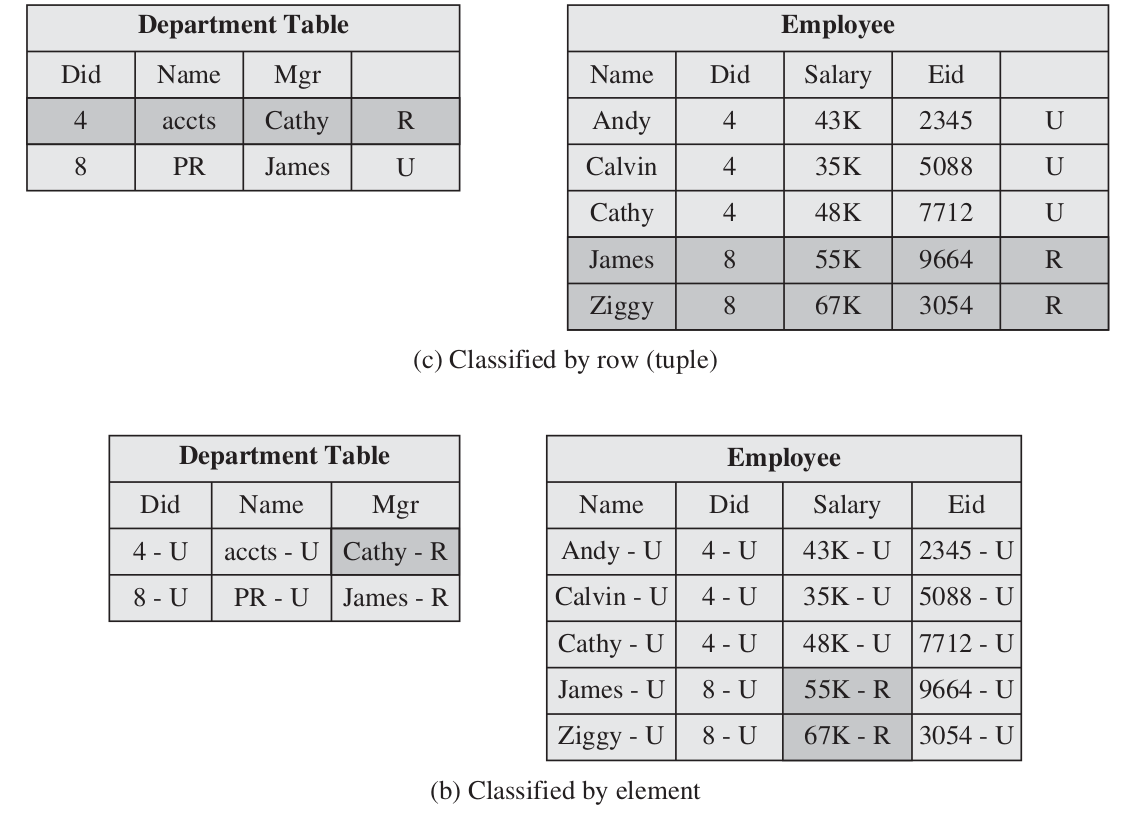
\includegraphics[width=0.8\linewidth]{database2}
  \end{center}
}
\end{frame}

\begin{frame}{MLS, databases and read}
  \begin{itemize}
  \item DBMS enforces simple security rule (no read up) 
  \item easy for database/table granularity
  \item inference problems if have column granularity
    \begin{itemize}
    \item if can query on restricted data can infer its existence 
    \item SELECT name FROM Employee WHERE Salary $>$ 50K 
    \item solution is to check access to all query data 
    \end{itemize}
  \item also have problems if have row granularity 
    \begin{itemize}
    \item null response in join queries can indicate restricted/empty result 
    \end{itemize}
  \end{itemize}
\end{frame}


\begin{frame}{MLS, databases and write}
  \begin{itemize}
  \item enforce *-security rule (no write down) 
  \item have problem if a low clearance user wants to 
    insert a row with a primary key that already exists 
    in a higher level row:
    \begin{itemize}
    \item can reject, but user knows row exists 
    \item can replace, compromises data integrity 
    \item can polyinstantiation and insert multiple rows with same 
      key, creates conflicting entries
    \end{itemize}
  \item same alternatives occur on update 
  \item avoid problem if use database / table granularity
  \end{itemize}
\end{frame}


\begin{frame}{Prove security: state space analysis}
  \begin{itemize}
  \item Map the design/implementation to the security model
    \begin{itemize}
      \item map states
      \item map transitions
    \end{itemize}
  \item $R$ = the set of states reachable by transitions from a
    (set of) initial state(s) $\star$
  \item $P$ = the set of authorized states (the three properties hold)
  \item System secure if $R \subseteq P$
  \item System insecure if $\exists S \in R. S \not \in P$
  \end{itemize}
  \only<2> {
  \begin{center}
    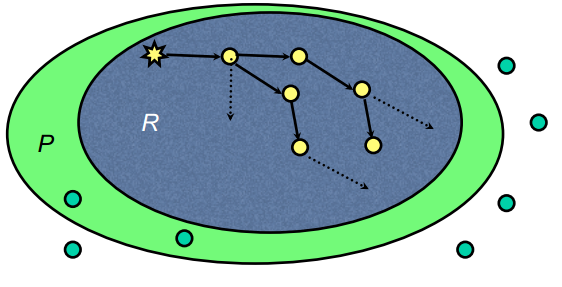
\includegraphics[width=0.5\linewidth]{secure_system}
  \end{center}}
  \only<3> {
  \begin{center}
    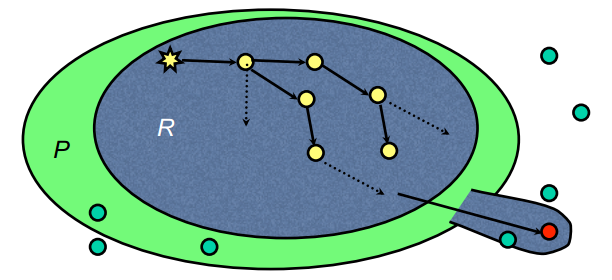
\includegraphics[width=0.5\linewidth]{insicure_system}
  \end{center}}
\end{frame}

\begin{frame}{Prove security: state space analysis}
  \begin{itemize}
  \item for all $\star \rightarrow p_1 \rightarrow \dots p_n$ holds
    $\{\star, p_1, \dots, p_n\} \subseteq P$
  \item State space analysis: model checking
  \item<2-> Prove that initial state $\star$ is secure 
  \item<3-> Show that each transition preserves security
  \item<4-> Ok for state-based properties
  \item<4-> Not enough for information flow properties
  \end{itemize}
\end{frame}

\begin{frame}[fragile]{Prove security: information flow properties}
  \begin{verbatim}
secret_key = 123456
program()
 secret_key = secret_key + 1
 public_var = 1
  \end{verbatim}
  \begin{itemize}
  \item Reason about knowledge
  \item<2-> $\{(pv=1, sk=123457)\} \subseteq P$
  \end{itemize}
\end{frame}

\begin{frame}[fragile]{Prove security: information flow properties}
  \begin{verbatim}
secret_key = 123456
program()
 secret_key = secret_key + 1
 public_var = secret_key
  \end{verbatim}
  \begin{itemize}
  \item Reason about knowledge
  \item<2-> $\{(pv=sk, sk=123457)\} \not \subseteq P$
  \end{itemize}
\end{frame}

\begin{frame}[fragile]{Prove security: information flow properties}
  \begin{verbatim}
secret_key = 123456
program()
 secret_key = secret_key + 1
 public_var = random()
  \end{verbatim}
  \begin{itemize}
  \item Reason about knowledge
  \item<2-> $\{(pv=1, sk=123457), (pv=2, sk=123457), \dots ,
    (pv=123457, sk=123457), \dots\} \subseteq P$
  \end{itemize}
\end{frame}

\begin{frame}[fragile]{Prove security: information flow properties}
  \begin{verbatim}
secret_key = 123456
program()
 secret_key = secret_key + 1
 if (secret_key mod 2 == 0)
   public_var += 42
  \end{verbatim}
  \begin{itemize}
  \item Reason about knowledge
  \item<2-> State based properties are not enough
  \end{itemize}
\end{frame}

\begin{frame}{Prove security: hyperproperties}
  \begin{itemize}
  \item let $H$ (high) be the classified variables
  \item let $L$ (low) be the public variables
  \item for every execution $\star \rightarrow p_1 \rightarrow \dots p_n$
  \item if $L(\star) = L(\star')$ then
  \item there is an execution  $\star' \rightarrow p'_1 \rightarrow \dots p'_n$
  \item such that $L(p_i) = L(p'_i)$
  \end{itemize}
\end{frame}

\begin{frame}[fragile]{Prove security: hyperproperties}
  \begin{itemize}
  \item for every execution $\star \rightarrow p_1 \rightarrow \dots p_n$
    if $L(\star) = L(\star')$  then there is an execution
    $\star' \rightarrow p'_1 \rightarrow \dots p'_n$
  such that $L(p_i) = L(p'_i)$
  \end{itemize}
  \begin{verbatim}
secret_key = 123456, secret_key' = 654321
program()
 secret_key = secret_key + 1
 public_var = 1
  \end{verbatim}
\end{frame}

\begin{frame}[fragile]{Prove security: hyperproperties}
  \begin{itemize}
  \item for every execution $\star \rightarrow p_1 \rightarrow \dots p_n$
    if $L(\star) = L(\star')$  then there is an execution
    $\star' \rightarrow p'_1 \rightarrow \dots p'_n$
  such that $L(p_i) = L(p'_i)$
  \end{itemize}
  \begin{verbatim}
secret_key = 123456, secret_key' = 654321
program()
 secret_key = secret_key + 1
 public_var = random()
  \end{verbatim}
\end{frame}

\begin{frame}[fragile]{Prove security: hyperproperties}
  \begin{itemize}
  \item for every execution $\star \rightarrow p_1 \rightarrow \dots p_n$
    if $L(\star) = L(\star')$  then there is an execution
    $\star' \rightarrow p'_1 \rightarrow \dots p'_n$
  such that $L(p_i) = L(p'_i)$
  \end{itemize}
  \begin{verbatim}
secret_key = 123456, secret_key' = 654321
program()
 secret_key = secret_key + 1
 if (secret_key mod 2 == 0)
   public_var += 42
  \end{verbatim}
\end{frame}

\begin{frame}{Trusted system}
  \begin{itemize}
  \item Trusted system:
    \begin{itemize}
    \item systems that is relied upon to a specified extent to enforce a specified security policy
    \end{itemize}
  \item Chain of trust
    \begin{itemize}
    \item is established by validating each component of hardware/software/data from the bottom up
    \end{itemize}
  \end{itemize}
\end{frame}

\begin{frame}{Secure boot}
  \begin{itemize}
  \item boot chain
    \begin{itemize}
      \item Boot ROM $S_0$ executes, then loads and starts BIOS
      \item BIOS $S_1$ executes, then loads and starts Boot Loader
        (e.g. GRUB)
      \item Boot loader $S_2$
      \item Kernel $S_3$
      \item SATA/SCSI driver
      \item Ext4/NTFS driver
      \item ....
\only<1>{
      \item Login service
      \item Shell
      \item Chrome
      \item Plug in
}
    \end{itemize}
   \item<2-> each stage $S_i$
     
     \begin{itemize}
       \item holds a public key $PU_i$
       \item is shipped with a certificate $cert_{i}$
         signed with $PR_{i-1}$
       \item measure $S_{i+1}$ by computing the hash of the
         code of $S_{i+1}$
       \item executes $S_{i+1}$ only if $SHA(S_{i+1}) = Dec(PU_i, cert_{i+i})$
     \end{itemize}
  \end{itemize}
\end{frame}



\begin{frame}{Trusted Platform Module}
  \begin{itemize}
  \item secure coprocessor that stores cryptographic keys and
    implement crypto functionality
  \item key assumption: the coprocessor is tamper proof
  \item TPM endorsement key: a unique RSA key burned into the chip
    during its production
  \item Disk encryption
  \item Video output only to trusted screen 
  \item Etc..
  \end{itemize}
\end{frame}

\begin{frame}{TPM: Secure boot}
  \begin{itemize}
  \item boot chain
    \begin{itemize}
      \item Boot ROM $S_0$ executes, then loads and starts BIOS
      \item BIOS $S_1$ executes, then loads and starts Boot Loader
        (e.g. GRUB)
      \item Boot loader $S_2$
      \item Kernel $S_3$
      \item SATA/SCSI driver
      \item Ext4/NTFS driver
      \item ....
    \end{itemize}
   \item TPM provide the key $PU_0$
  \end{itemize}
\end{frame}

\begin{frame}{TPM: Authenticated boot, remote attestation}
  \begin{itemize}
  \item boot chain
    \begin{itemize}
      \item Boot ROM $S_0$ executes, then loads and starts BIOS
      \item BIOS $S_1$ executes, then loads and starts Boot Loader
        (e.g. GRUB)
      \item Boot loader $S_2$
      \item Kernel $S_3$
      \item SATA/SCSI driver
      \item Ext4/NTFS driver
      \item ....
    \end{itemize}
   \item each stage $S_i$
     \begin{itemize}
       \item measure $S_{i+1}$ by computing the hash of the executable
         code of $S_{i+1}$
       \item asks to the TPM to append to the log $LOG_{i+1} =
         SHA1(LOG_{i} | S_{i+1} | nonce)$
       \item the log can be signed with the TPM key
     \end{itemize}
  \end{itemize}
\end{frame}

\begin{frame}{TPM: Encryption service}
  \begin{itemize}
  \item TPM keeps an additional master key $(PU_m, PR_m)$ that is
    unique for the machine 
  \item TPM generates a configuration key $(PU_c, PR_c)$ that depends
    on the log $LOG$ and the master key
  \item this key can be used to encrypt data that can be decrypted
    only by the machine with the actual configuration
  \item TPM can generate a key pair for $S_i$, the public key is used
    to encrypt DRM content that can only be played on this machine and
    by the SW $S_i$
  \end{itemize}
\end{frame}


\begin{frame}{TPM: Criticism}
  \begin{itemize}
    \item Not only protects the user but also from the user
    \item Depends on the endorsement key is burned into the
      chip at the manufacturing plant
      
      \begin{itemize}
      \item manufacturer must have had access to the private key at least
        during the time of manufacturing
      \item The user
        will have to blindly trust the manufacturer
      \item  the company that
        designed the chip
      \item those companies allowed to make software
        for the chip
      \item the authorities
      in the country where the chip was manufactured
      \item usage of Physically Unclonable Function
      \end{itemize}
      
    \item Users unable to exercise legal rights: e.g. legal backups
    \item Users vulnerable to vendor withdrawal of service
  \end{itemize}
\end{frame}

\begin{frame}{Concluding remarks}
  \begin{itemize}
    \item Models to reason about security (BLP/Chinese Wall)
    \item Applicable to several scenarios
    \item Enforcement methodologies/techniques
  \end{itemize}
\end{frame}

\end{document}

%%% Local Variables: 
%%% mode: latex
%%% TeX-master: t
%%% End: 
